%chapappratus.tex
%
The experiment was performed at the Thomas Jefferson National Accelerator Facility (Jefferson Lab) in Newport News, Virginia. The electron accelerator is known as the Continuous Electron Beam Accelerator Facility (CEBAF) and is capable of probing nucleon and quark structure in nuclei.

%
\Section{TJNAF Overview}%
%
An aerial view of Jefferson Lab is shown in \figureref{jlab}. Currently there are three halls using the continuous electron beam from the accelerator. The three halls (namely Hall-A, Hall-B and Hall-C) are shown in \figureref{jlab} by three RED circles from left to right respectively. In the future, JLab will upgrade it's energy from 6 GeV to 12 GeV, and a new hall (Hall-D) will be added, as shown in \figureref{beamline}.

%\begin{figure}[!tbp]
%\begin{center}
%  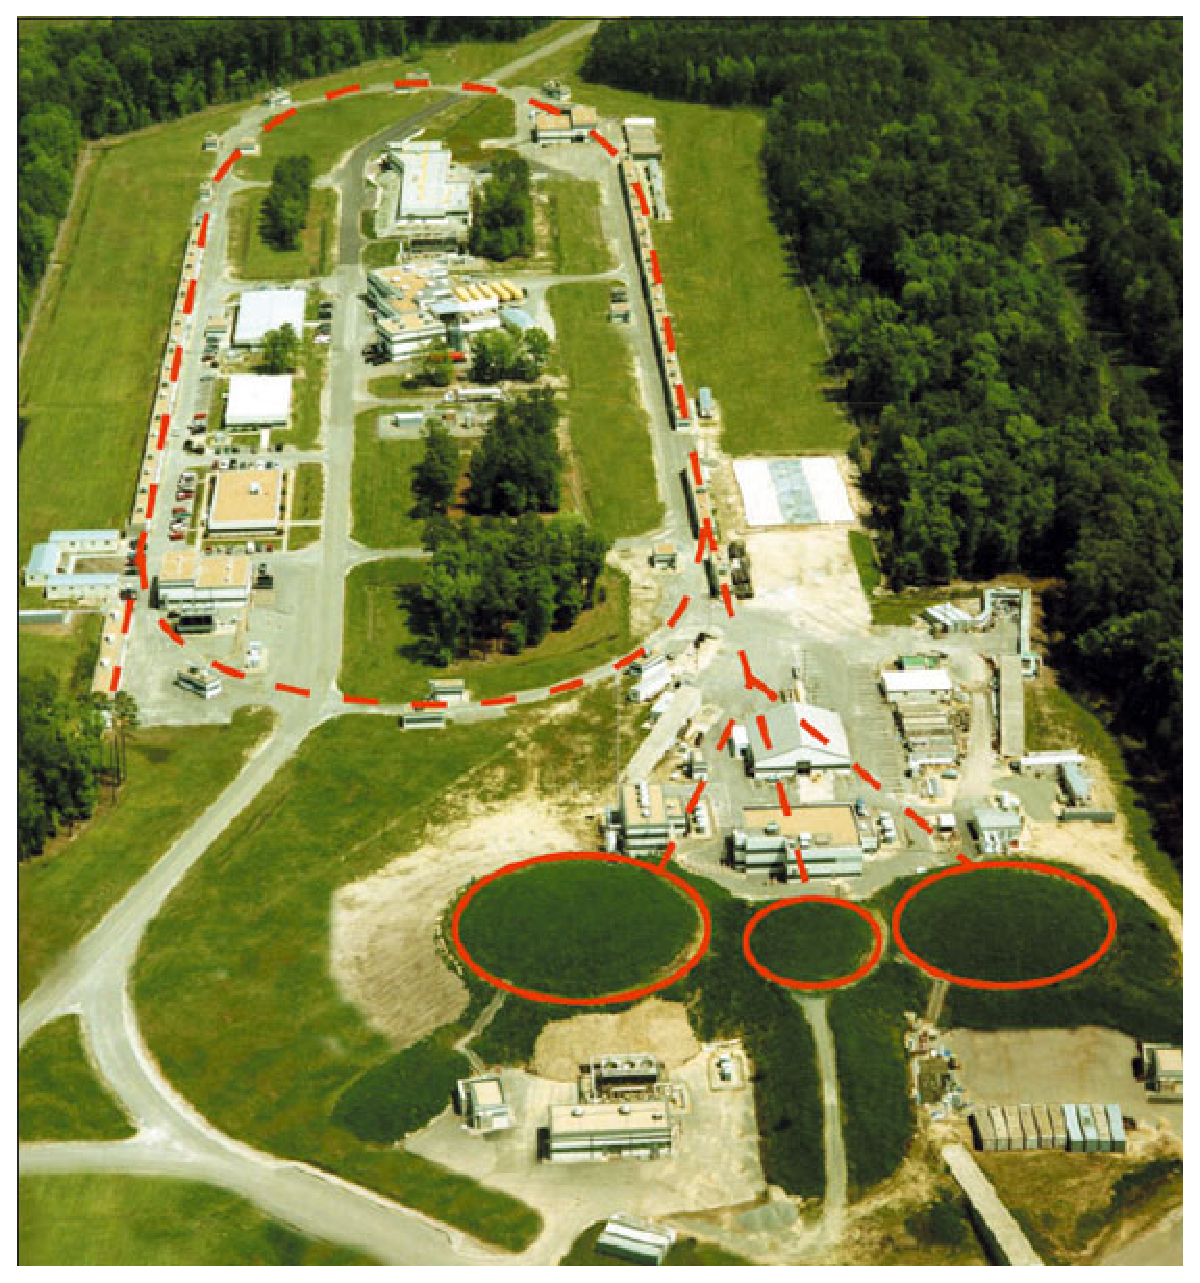
\includegraphics[width=1.0\columnwidth]{jlab}
%  \caption[Aerial view of Jefferson Lab \cite{jlab}.]{\label{fig:jlab}Aerial view of Jefferson Lab \cite{jlab}.}
%\end{center}
%\end{figure}
\setlength{\figwidth}{1.0\linewidth}
\Figure{jlab}{\figwidth}{Aerial view of Jefferson Lab \cite{jlab}.}

%\setlength{\figwidth}{0.9\linewidth}
%\Figure{cointime}{\figwidth}{cointime}

%
\Section{Accelerator}%
\label{Accelerator}
The length of the accelerator is about 7/8 of a mile for one complete cycle. A polarized electron source at the injector is used to extract electron beam of energy 45 MeV with the standard setup of JLab. The electron beam is accelerated by two linear accelerators, north and south linacs. A series of magnets bends the beam along the arcs which connects the two linacs. The beam line, transporting the beam to the three halls is shown in \figureref{beamline} by the RED lines. The continuous-wave (100\% duty factor) electron beam from the CEBAF accelerator has a characteristic 2 ns micro-structure that arises from the 1.5 GHz radio frequency (RF) structure of the accelerator and the 499 MHz three-hall beam splitting scheme. 

\SubSection{Polarized Source}%
\label{Polarized Source}
The production and acceleration of the electron beam starts with a polarized electron source. Circularly polarized light produces polarized electrons from a strained super-lattice gallium arsenide (GaAs) cathode through photoemission. This cathode is made up of several layers of material containing GaAs with varying amounts of phosphorus doping, grown on a substrate.

\SubSection{LINAC}%
\label{LINAC}
Electrons from the injector are sent to the north linear accelerator (linac) at an energy of 45 MeV. Superconducting niobium RF resonant cavities in the north linac section accelerate the electrons; in a standard tune, the maximum gain in energy per linac is 600 MeV in energy. The beam then goes through the east arc and into the south linac to be accelerated for another 600 MeV energy gain. This beam can be sent directly to the Beam Switch Yard (BSY) for distribution to the experimental halls or the beam can be steered along the west arc for another pass through the two linacs for another 1.2 GeV of energy gain. This process can be repeated up to four times. A maximum of five passes  through both linacs provide energies from 445 MeV to 5945 MeV. As the beam energies are different in each pass, a different set of magnets are used to steer the beam around the arcs after each pass.

\begin{figure}[!tbp]
  \centering
  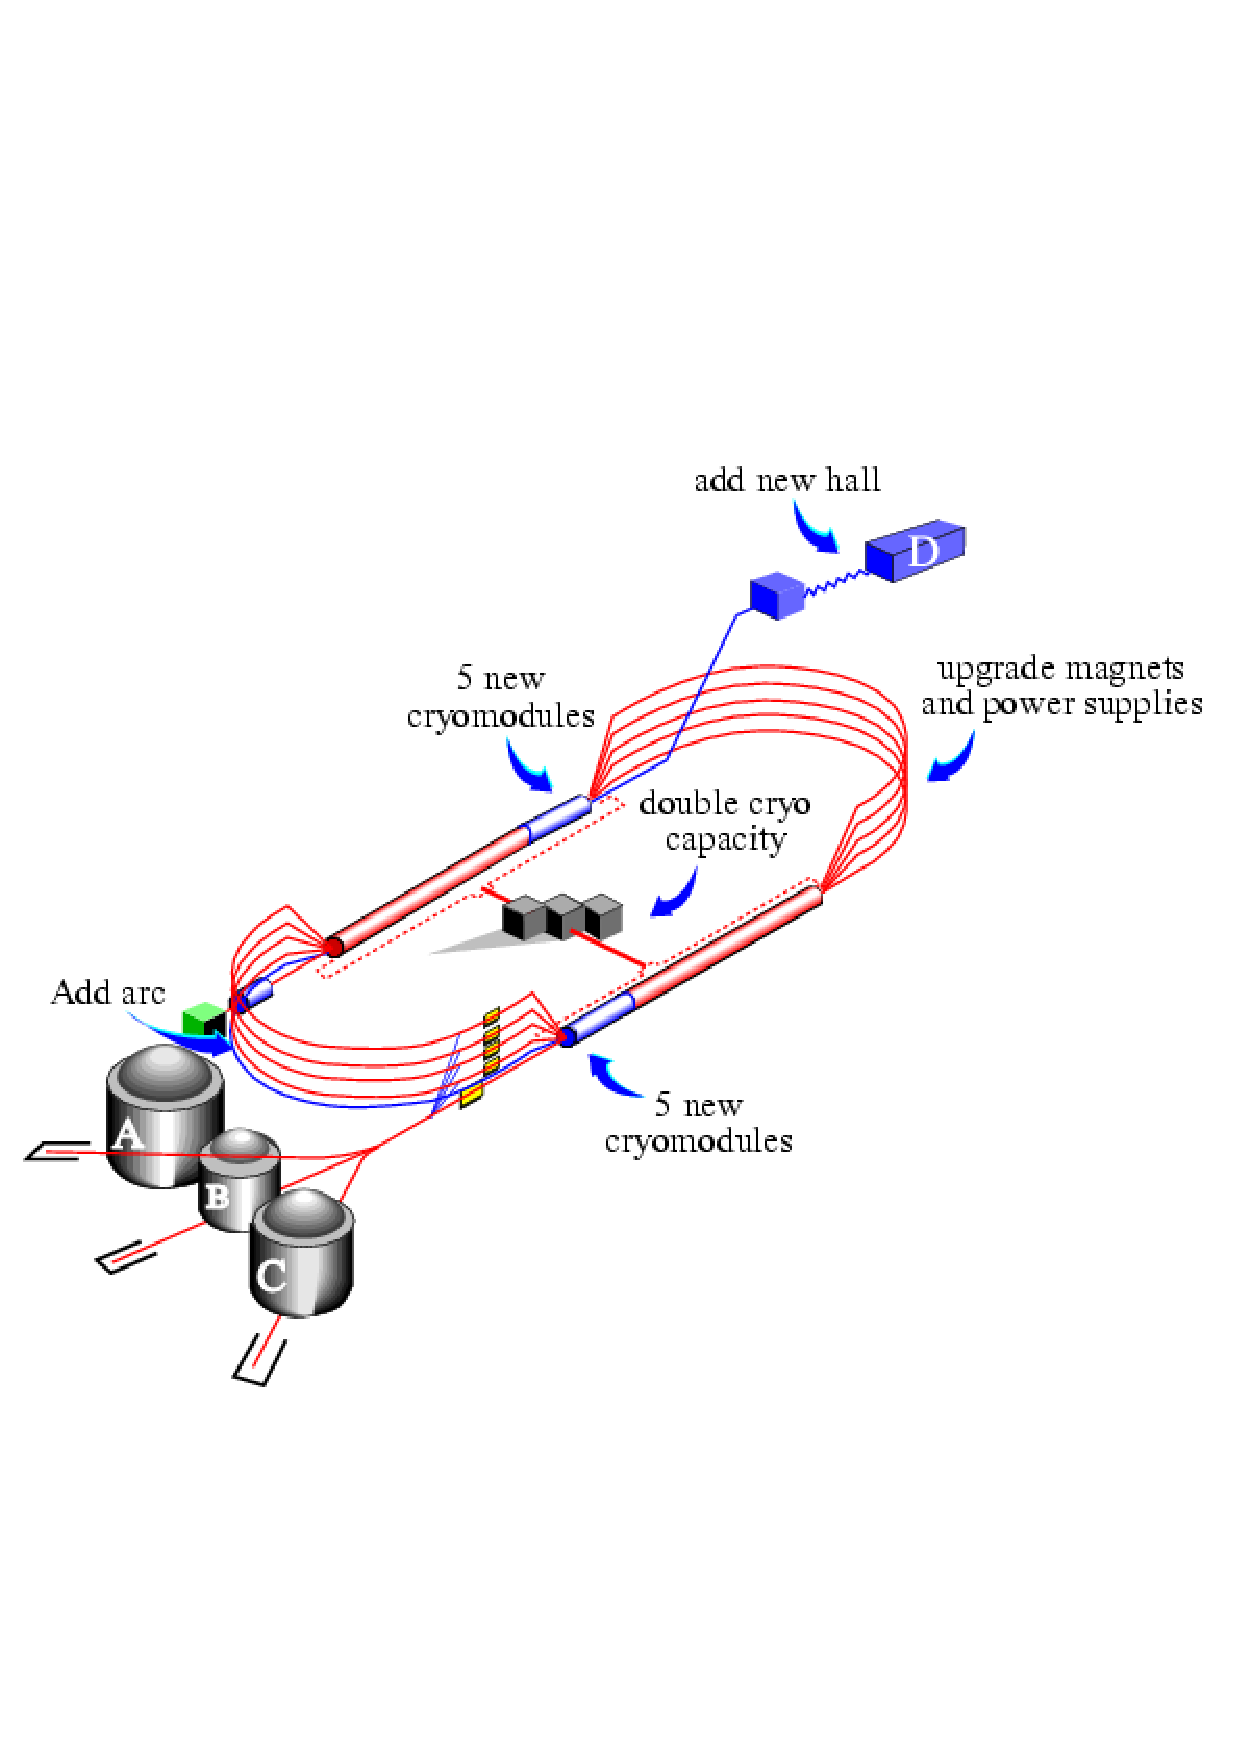
\includegraphics[trim = 0mm 57mm 0mm 50mm,clip,width=1.0\columnwidth]{beamline}
  \caption[Schematic of Jefferson Lab.]{\label{fig:beamline}Schematic of Jefferson Lab.\\\\ Beam is accelerated by two linear accelerator namely north linac and south linac. Three existing Halls A, B, C and one under construction, Hall-D, are shown. The new components that would be added for 12 GeV energy upgrade are also shown in the picture.}
\end{figure}
%\setlength{\figwidth}{0.9\linewidth}
%\Figure{beamline}{\figwidth}{Schematic of Jefferson Lab: Beam is accelerated by two linear accelerator namely north linac and south linac. Three existing Halls A, B, C and one under construction, Hall-D, are shown. The new components that would be added for 12 GeV energy upgrade are also shown in the picture.}
\Section{Beamline}%
\label{Beamline}
The beamlines that transport the beam from the accelerator to the experimental halls  is shown in \figureref{beamline}. Each beamline consists of a series of quadrupole and dipole magnets to help focus/ defocus the beam along the way to the target in each hall.

%Beamline of the Jefferson Lab has been shown in the \figureref{beamline}. The projected beamline of Hall-D and new cryogenic modules for 12 GeV upgradation are also shown in the figure. A series of powerful quadrupoles and dipoles are used along the beamline to focus and defocus the beam along the beamline. A two meter long dipole splits the beam for three diffrent halls.

\SubSection{Hall-C Beamline}
\label{Hall-C Beamline}
The beam position, profile and current were measured at various points along the Hall-C beamline. A part of Hall-C beamline also forms an arc. The bending magnets of the Hall-C arc can be used to measure the relative beam energy with a precision of $\Delta$E/E $\approx$ $10^{-4}$.

\SubSection{Beam Position Monitor}%
\label{Beam Position Monitor}
The beam position was continuously monitored by beam position monitors (BPM) during data collection to ensure that the beam was centered on the target. The transverse beam size was 60-130 $\mu$m in diameter and was measured by a superharp (pair of wires that can be moved in and out of the beam) scanner. The BPMs and superharps could measure the beam position with a precision of 0.2 $mm$ and 0.01 $mm$, respectively \cite{BC06}.

\SubSection{Beam Current Monitor}%
\label{Beam Current Monitor}
The beam current was monitored through a combination of a parametric DC current transformer (Unser monitor) and coupled cylindrical resonant cavities(Beam Current Monitor 1 and 2) which provided a continuous relative measurement of the current during each data run \cite{BC06,RM99}.

\SubSection{Raster}%
For liquid targets, the beam was rastered over an area of the target of up to 2x2 mm$^2$ by the Fast Raster to reach acceptable beam currents without damaging the target and to reduce the effect of localized boiling in the liquid targets.
%Slow raster was used to decrease the power density of the beam before the beam dump to reduce the damage.

\Section{Hall-C}%
\label{Hall-C}
The E01-107 experiment was performed in the Hall-C. Hall-C is shown in \figureref{HALC_33}. One can see the beamline is going to the target. There is a Short Orbit Spectrometer (SOS) on the left to collect scattered electrons and a High Momentum Spectrometer (HMS) to collect hadrons on the right at the far end. The unscattered beam is dumped in the Beam Dump at the other end of the hall. 
%The dimensions of the components can be realized by looking the scientist stnding on the left near Short Orbit Spectrometer hut.
%\begin{figure}[!tbp]
%  \centering
%  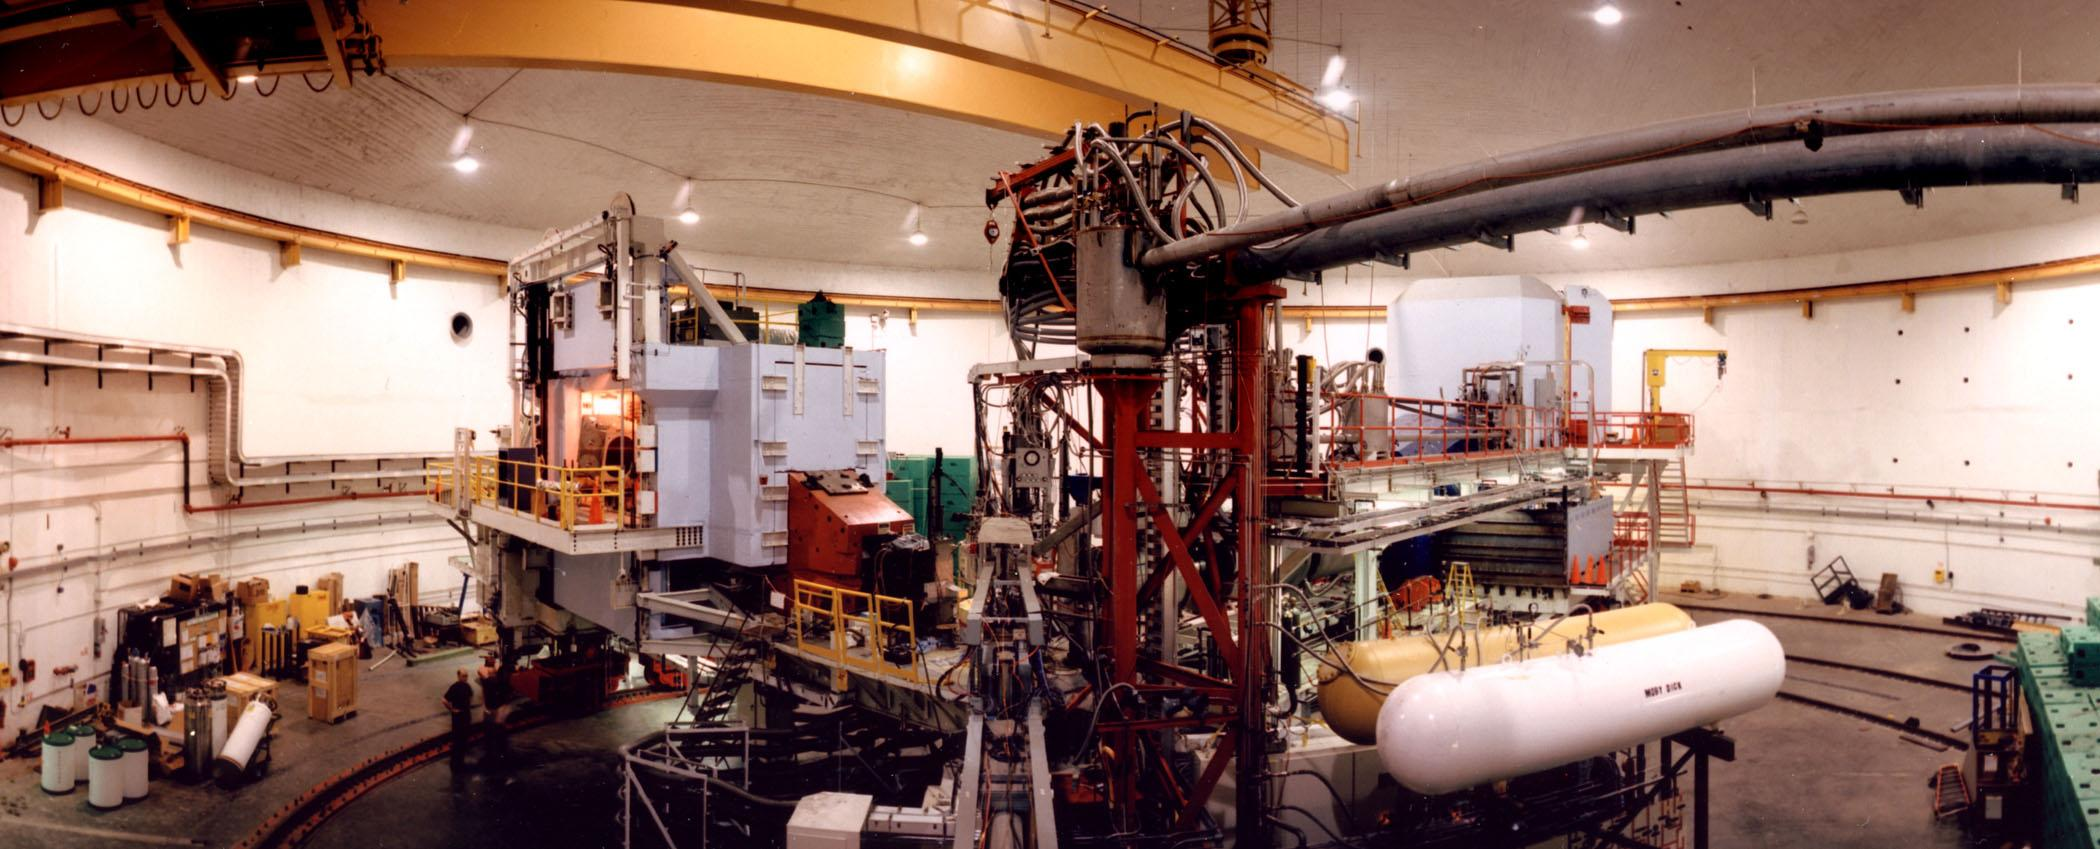
\includegraphics[width=1.0\columnwidth]{HALC_33}
%  \caption[Hall C at Jefferson Lab.]{\label{fig:HALC_33}Hall C at Jefferson Lab.}
%\end{figure}

\setlength{\figwidth}{1.0\linewidth}
\Figure{HALC_33}{\figwidth}{Hall C at Jefferson Lab.}

\SubSection{Short Orbit Spectrometer (SOS)}%
\label{SOS}
The Short Orbit Spectrometer uses three room temperature magnetic elements: a quadrupole followed by two dipoles (QDD) as shown in \figureref{sos} \cite{GaskelD}. The SOS can be rotated about the target in order to detect scattered particles at different scattering angles. In this experiment, scattered electron were detected in the SOS. The configuration of the detectors in the SOS is discussed in Section \ref{Detector Packages}.

\begin{figure}[tbp]
  \centering
  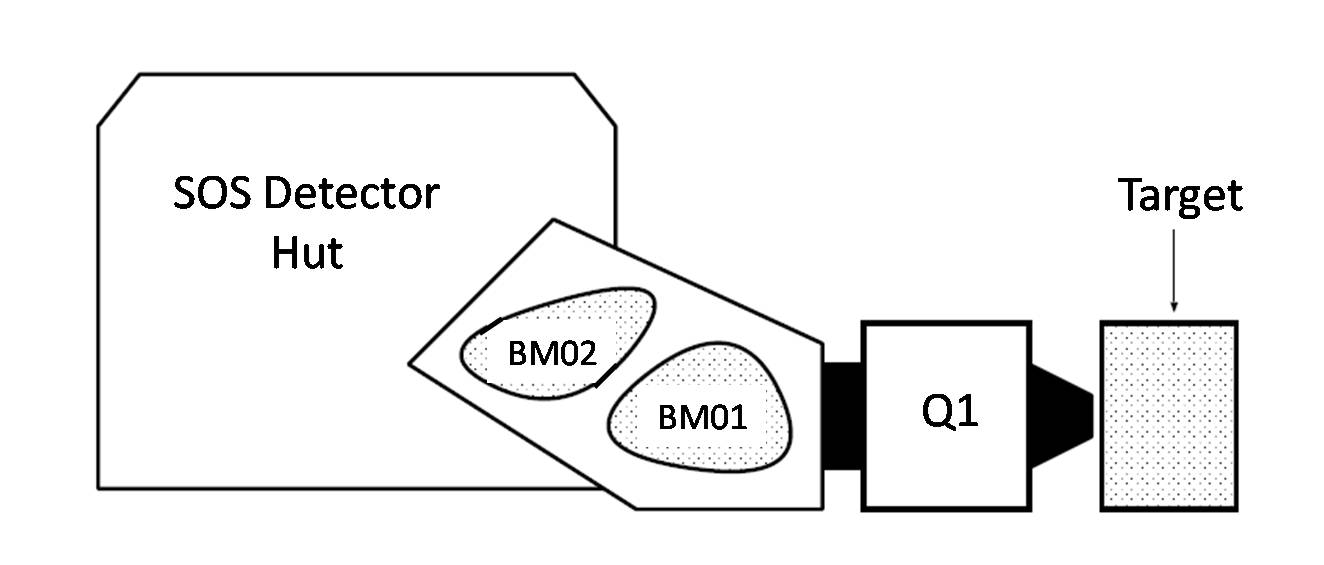
\includegraphics[trim = 0mm 4mm 2mm 0mm,clip,width=0.9\columnwidth]{sos}
  \caption[Side view of SOS \cite{GaskelD}.]{\label{fig:sos}Side view of SOS \cite{GaskelD}.}
\end{figure}
%\setlength{\figwidth}{0.8\linewidth}
%\Figure{sos}{\figwidth}{Side view of SOS \cite{GaskelD}.}

\SubSection{High Momentum Spectrometer (HMS)}%
\label{HMS}
The High Momentum Spectrometer is composed of four superconducting magnetic elements in order to focus and separate different particles based on their momentum and charge. In our experiment, $\pi^+$, $K^+$ and protons were detected in the HMS. The magnetic elements consisted of three quadrupoles followed by a dipole (QQQD) is shown in \figureref{hms} \cite{GaskelD}. The HMS can be rotated about the target as well. The configuration of the detectors in the HMS is discussed in Section \ref{Detector Packages}.

\begin{figure}[tbp]
  \centering
  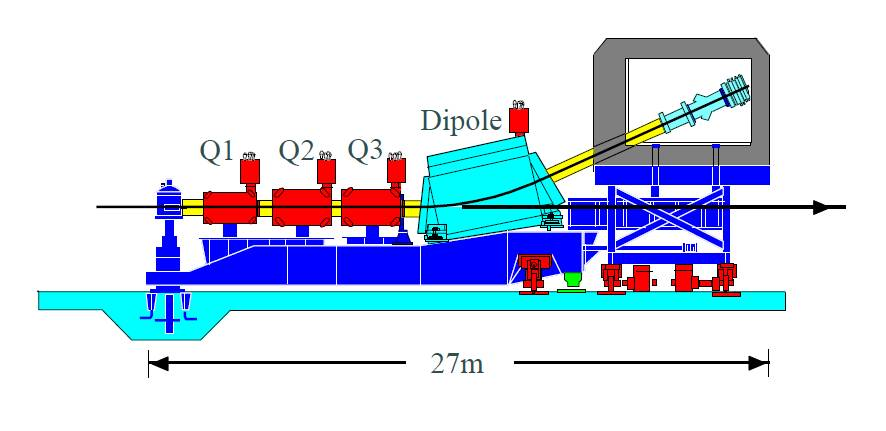
\includegraphics[trim = 0mm 10mm 2mm 0mm,clip,width=1.0\columnwidth]{hms}
  \caption[Side view of HMS \cite{GaskelD}.]{\label{fig:hms}Side view of HMS \cite{GaskelD}.}
\end{figure}
%\setlength{\figwidth}{1.0\linewidth}
%\Figure{hms}{\figwidth}{Side view of HMS \cite{GaskelD}.}

\SubSection{Target}%
\label{Target}
The electron beam with energy of up to 5.8 GeV was incident on liquid hydrogen and deuterium, and solid foil targets of $^{12}$C, $^{27}$Al, $^{63}$Cu, and $^{197}$Au. For the cryotargets, a 4.0 cm diameter cylindrical cell with an axis perpendicular to the beam direction was used. The cell walls with a thickness of 0.01 cm were made from an aluminum alloy. A schematic diagram of the cryogenic target ladder are shown in \figureref{target}. The target ladder could be translated vertically by lifter motors.

\begin{figure}[tbp]
  \centering
  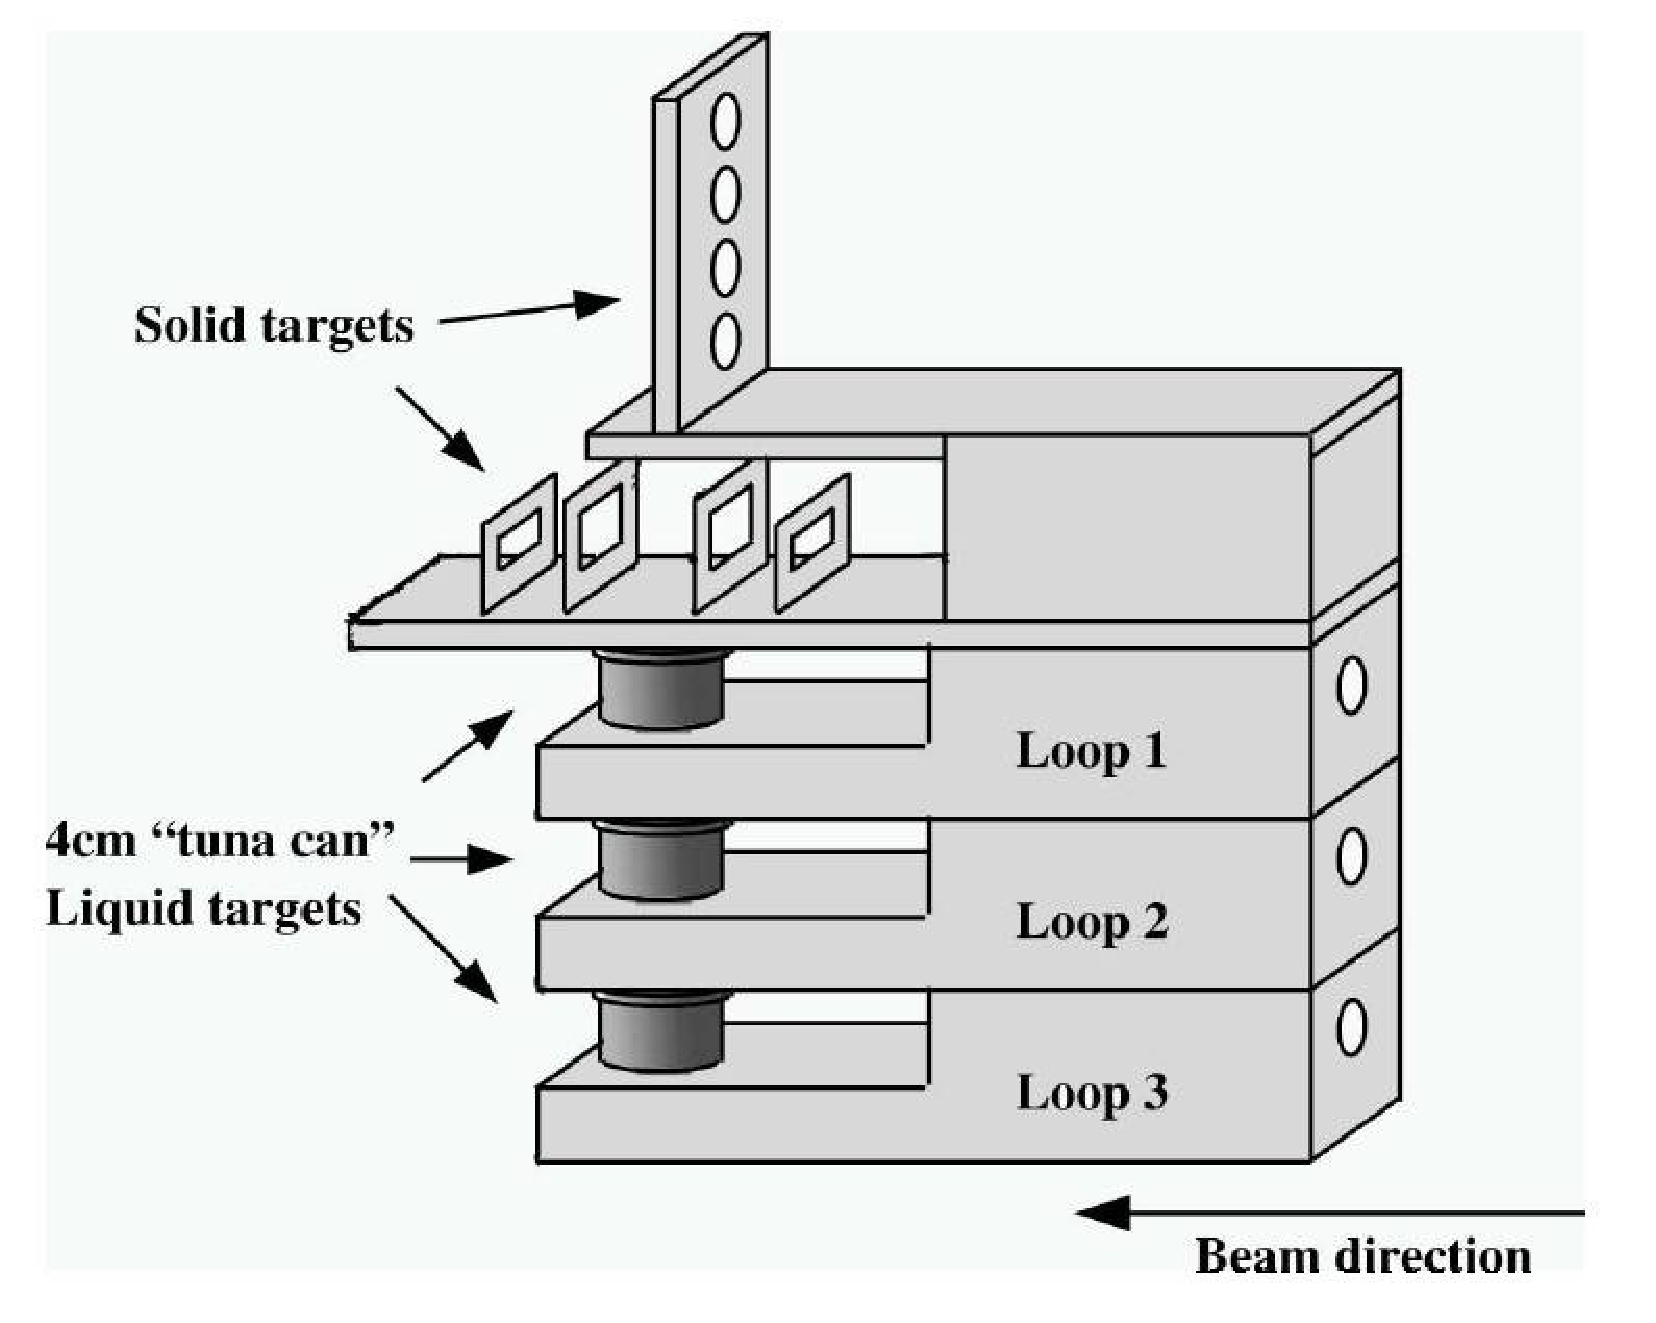
\includegraphics[width=0.8\columnwidth]{target}
  \caption[Schematic diagram of target ladder \cite{BC06}.]{\label{fig:target}Schematic diagram of target ladder \cite{BC06}.}
\end{figure}
%\setlength{\figwidth}{0.7\linewidth}
%\Figure{target}{\figwidth}{Schematic diagram of target ladder \cite{BC06}.}

\SubSection{Detector Packages}%
\label{Detector Packages}
There are two wire chambers each in the HMS and SOS, separated by 81.5 cm in the HMS and by 49.5 cm in the SOS to determine the position and angle of a track. Each wire chamber has six planes of wires and a 1:1 gas mixture of argon and ethane are surrounding the wires. The position resolutions of the HMS and SOS drift chambers were 280 $\mu$m and 180 $\mu$m, respectively \cite{BC06, hinton01}.

Four planes of scintillator hodoscopes are used both in the HMS and in the SOS to form the primary trigger for charged particle detection. These four planes were used to identify a particle that passed through them and produced signals.

$\breve{C}$erenkov detectors were used to detect the $\breve{C}$erenkov radiation emitted when a particle enters a medium and moves faster than the speed of light in that medium. Two types of $\breve{C}$erenkov detectors were used for particle identification (PID): Aerogel $\breve{C}$erenkov and Gas $\breve{C}$erenkov. Silica aerogel $\breve{C}$erenkov of refractive index n = 1.015 with threshold for $\pi^+$ of 0.8 GeV/c and a threshold for $K^+$ of 2.85 GeV/c was used; this allowed us to separate particles traveling above and below the threshold. A gas $\breve{C}$erenkov detector filled with 0.956 atm of perfluorobutane ($C_4F_{10}$) with an index of refraction of 1.0015 and a momentum threshold of 2.65 GeV/c for $\pi^+$ and threshold of 9.4 GeV/c for $K^+$ was used for PID as well \cite{BC06}.

%
\Section{Data Acquisition}%
\label{Data Acquisition}
The CEBAF Online Data Acquisition (CODA) software system managed real time reading of the data, its storage to disk as well as user interface \cite{Abb95}. Read Out Controller (ROC) CPUs managed the readout electronics, ADCs, TDCs and scalers. CODA software also read the ROCs directly via a parallel link over an ethernet network and wrote each event onto disk. Information about the beam position, magnet settings, target status and accelerator status were read out every 30 seconds using Experimental Physics Industrial Control System (EPICS) software \cite{RM99}.

%
\Section{Kinematic Settings}%
\label{Kinematic Settings}%
The E01-107 experiment was carried out in Hall C at Jefferson Lab \cite{CW01} in 2004. The kinematic settings of the measurements are shown in \Tableref{kine}. The experiment was designed to measure the nuclear transparency of pions using the ($e,e^\prime \pi^+$) reaction for five kinematic settings of $Q^2$ = 1.1, 2.15, 3.0, 3.91 and 4.69 $\mathrm{(GeV/c)^2}$. In addition to pions a reasonable sample of kaons were also recorded in the 30 ns coincidence window. The kaon statistics were very low for $Q^2$ = 3.91 and 4.69 $\mathrm{(GeV/c)^2}$ kinematic settings, hence this analysis covers only three kinematic settings, as listed in \Tableref{kine}.

More details of the experimental apparatus can be found in references \cite{BC06, RM99, hinton01}.

\begin{table}
  \caption[The central kinematics of the experiment.]{\label{tab:kine}The central kinematics of the experiment.}
\begin{center}
%\centering
\label{table1}
\begin{tabular}{||c|c|c|c|c|c|c|c||}\hline
 $Q^2$ & $-t$ & $E_e$ & $\theta_{e^\prime}^{\rm SOS}$ &$E_{e^\prime}$ &
 $\theta_{K^+}$ & $\theta_{\rm HMS}$ & $p_{K^+}$ \\
 (GeV/c)$^2$ & (GeV/c)$^2$ & GeV & deg & GeV & deg & deg & GeV/c \\\hline
1.10 &0.050 &4.021 &27.76 &1.190 &10.58 &10.61 &2.793 \\
2.15 &0.158 &5.012 &28.85 &1.730 &13.44 &13.44 &3.187 \\
3.00 &0.289 &5.012 &37.77 &1.430 &12.74 &12.74 &3.418 \\\hline
\end{tabular}
\vspace{-0.5cm}
\end{center}
\end{table}
%\Table{kine}{The central kinematics of the experiment.}
